\newcommand{\din}[0]{\ensuremath{\delta_{in}}}
\newcommand{\dout}[0]{\ensuremath{\delta_{out}}}

%%%%%%%%%%%%%%%%%%%%%%%%%%%%%%%%%%%%%%%%%%%%%%%%%%%%%%%%%%%%%%%%%%%%%%%%%%%%%%
%%%%%%%%%%%%%%%%%%%%%%%%%%%%%%%%%%%%%%%%%%%%%%%%%%%%%%%%%%%%%%%%%%%%%%%%%%%%%%
%%%%%%%%%%%%%%%%%%%%%%%%%%%%%%%%%%%%%%%%%%%%%%%%%%%%%%%%%%%%%%%%%%%%%%%%%%%%%%

\section{Introduction} \label{sec:introduction}

Large software systems need to be decomposed in modules in order to be
effectively maintained by groups of developers working concurrently. Software
clustering algorithms \cite{Anquetil1999}, also known as architecture recovery
algorithms, find suitable decompositions by analyzing the dependencies between
components in a software system (e.g., classes in object-oriented systems) and
then grouping together highly interdependent components.

Although many software clustering algorithms have been proposed, there is
little empirical evaluation regarding the external quality of the
decompositions they find, i.e., how close the decompositions are from reference
decompositions made by experienced developers \cite{Anquetil1999}. It is
expected that a good algorithm finds decompositions that are similar to
reference decompositions, which can be measured by a similarity metric such as
MoJo or EdgeSim \cite{Mitchell2001}.

Unfortunately, there are few publicly available reference decompositions
\cite{Anquetil1999} and, as a result, there are few studies that compare
software clustering algorithms. Also, because it is costly to obtain reference
decompositions for large systems, most studies test the algorithms with a
couple of small and medium systems \cite{Anquetil1999,Bittencourt2009}.

An alternative approach is to run the algorithms on synthetic, i.e., computer-
generated, component dependency networks with built-in reference
decompositions. This approach enables one to test algorithms with arbitrarily
large samples in a controlled manner. Nevertheless, this approach is often
overlooked, mainly because networks synthesized by naive random network models
are very dissimilar from real component dependency networks.

In this paper, we show that three recently proposed network models are capable
of synthesizing networks that resemble software component dependency networks.
For the sake of simplicity, we limit our analysis to networks of static
dependencies between classes in object-oriented systems written in Java.

The paper is organized as follows: Section \ref{sec:models} summarizes main
characteristics of the three network models.
%
Section \ref{sec:characterization} demonstrates a method to tell if a network
resembles a software component dependency network.
%
Section \ref{sec:evaluation} shows empirically that the three models synthesize
networks that resemble software component dependency networks.
%
Section \ref{sec:conclusion} discusses the impact of this research and future
work.

%%%%%%%%%%%%%%%%%%%%%%%%%%%%%%%%%%%%%%%%%%%%%%%%%%%%%%%%%%%%%%%%%%%%%%%%%%%%%%
%%%%%%%%%%%%%%%%%%%%%%%%%%%%%%%%%%%%%%%%%%%%%%%%%%%%%%%%%%%%%%%%%%%%%%%%%%%%%%
%%%%%%%%%%%%%%%%%%%%%%%%%%%%%%%%%%%%%%%%%%%%%%%%%%%%%%%%%%%%%%%%%%%%%%%%%%%%%%

\section{Network Models} \label{sec:models} 

Network theory studies general properties of many types of networks by using
statistical analysis. Of special interest are the so called scale-free
networks, i.e., networks with a highly heterogeneous distribution of the number
of edges per vertex. Scale-free networks have been found in many domains,
including sociology, biology, technology, linguistics, and software. It has
been found that class dependency networks, represented as directed unweighted
graphs, are scale-free \cite{Myers2003}. Thus, the study of the structure of
object-oriented software systems can benefit from the vast literature available
about scale-free networks.

Scale-free network models are algorithms that can be proven, either formally or
empirically, to synthesize networks that are scale-free. Although many
scale-free network models have been proposed, we were able to find in the
literature only two models that generate networks with built-in modules: CGW
\cite{Chen2008} and LFR \cite{Lancichinetti2009}. Also, we adapted a simple and
flexible model, BCR \cite{Bollobas2003}, to produce modules. We called the new
model BCR+.

The networks generated by the three models are represented as directed
unweighted graphs with modules, which makes them suitable for testing software
clustering algorithms. All models are controllable by a set of parameters,
including number of vertices and number of modules. Parameters specific to each
model influence network characteristics such as number of edges and proportion
of external edges (edges connecting vertices from distinct modules).

%%%%%%%%%%%%%%%%%%%%%%%%%%%%%%%%%%%%%%%%%%%%%%%%%%%%%%%%%%%%%%%%%%%%%%%%%%%%%%
%%%%%%%%%%%%%%%%%%%%%%%%%%%%%%%%%%%%%%%%%%%%%%%%%%%%%%%%%%%%%%%%%%%%%%%%%%%%%%
%%%%%%%%%%%%%%%%%%%%%%%%%%%%%%%%%%%%%%%%%%%%%%%%%%%%%%%%%%%%%%%%%%%%%%%%%%%%%%

\section{Characterization of Software Networks} \label{sec:characterization}

In the remaining of this paper, we will use the expression ``software network''
to refer to a network of static dependencies between classes of a software
system, in contrast to networks studied in other domains.

Our research hypothesis is that at least one of the presented models can
synthesize networks that are similar to software networks. A central issue,
thus, is how to measure similarity between networks.

We already know that the models synthesize networks that, just like software
networks, are scale-free. This single property, though, is insufficient to
prove the hypothesis, since many known scale-free networks are not software
networks (e.g., biologic networks). Therefore, the similarity metric should be
able to distinguish between software and non-software networks.

In this section we present a similarity metric and validate it by applying it
to a data set containing both software and non-software networks. 

%%%%%%%%%%%%%%%%%%%%%%%%%%%%%%%%%%%%%%%%%%%%%%%%%%%%%%%%%%%%%%%%%%%%%%
\subsection{Similarity Between Networks}

In a recent work, Milo et al. \cite{Milo2004} characterized networks by
analyzing their triad concentration. A triad is a network with three vertices
in which all vertices are connected. There are only 13 distinct triads, one for
each possible configuration of directed edges, as shown in Figure
\ref{fig:triads}.

\begin{figure}[t]
\centering
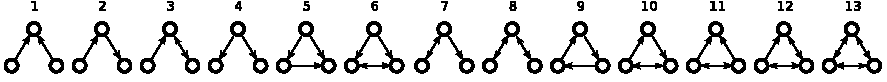
\includegraphics{triads}
%[width=1.0\textwidth]{triads}
\caption{The 13 network triads.}
\label{fig:triads}
\end{figure}

By counting how many times each triad appears in a network, one can build a
triad concentration profile (TCP), which is a vector with 13 numbers that
summarize the local structure of the network. Figure \ref{fig:profiles} shows
the TCP for networks from two distinct domains.

% Word adjacency network: word Y follows word X => X->Y
\begin{figure}[t]
\center
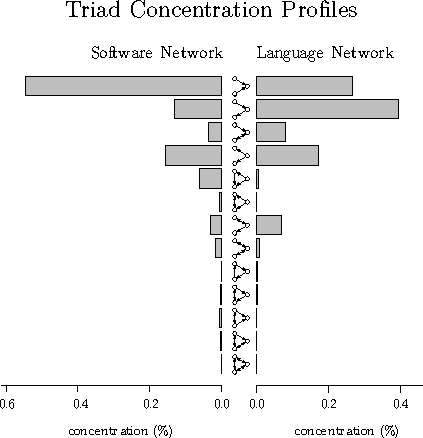
\includegraphics{tcp}
\caption{Triad concentration profiles (TCP) for two networks. On the left,
network extracted from the software system JabRef, version 2.5b2. On the
right, word adjacency network for the Japanese language \cite{Milo2004}.}
\label{fig:profiles}
\end{figure}

Following the work by Milo et al. \cite{Milo2004}, similarity between two
networks is measured by computing Pearson's correlation coefficient between the
corresponding TCPs, which yields a value between -1 (most dissimilar) and 1
(most similar):

$$
\mathrm{similarity}(a, b) ~=~ 
  \mathrm{cor}(\mathrm{TCP}(a), \mathrm{TCP}(b))\mathrm{,}
$$

where $a$ and $b$ are networks, TCP($x$) is the triad concentration profile for
network $x$, and cor($x$, $y$) is Pearson's correlation coefficient.

%%%%%%%%%%%%%%%%%%%%%%%%%%%%%%%%%%%%%%%%%%%%%%%%%%%%%%%%%%%%%%%%%%%%%%
\subsection{Data Set}

To support the evaluation of the metric, we have collected 131 networks from
many different domains. The networks are described in detail at
\url{http://bit.ly/7DPW5X}.

\subsubsection{Software networks} We have collected 65 software systems written
in Java, with size ranging from 111 to 35,363 classes. Java was chosen for
being a popular programming language in which many open source systems have
been written. The software networks, representing static dependencies between
classes, were extracted with the tool Dependency Finder
(\url{http://depfind.sf.net}).

\subsubsection{Non-software networks} We have collected 66 networks from
distinct domains, such as biology, sociology, technology, and linguistics, with
size ranging from 32 to 18,163 vertices. These networks are freely available on
the Internet and have been previously studied in the literature.
% S-score

%%%%%%%%%%%%%%%%%%%%%%%%%%%%%%%%%%%%%%%%%%%%%%%%%%%%%%%%%%%%%%%%%%%%%%
\subsection{Evaluation of the Similarity Metric}

%In order to evaluate the similarity metric, we measured the similarity between
%the networks in the data set. 

For the purposes of this research, a similarity metric must fulfill two
conditions: (i) it must yield high similarity between software networks, and
(ii) it must yield lower similarity between software networks and networks from
other domains.

Using the data set we can define S-score, a metric that represents how much a
particular network resembles software networks. It is defined as the average
similarity between the network and a sample of software networks:

$$
\mathrm{S\mbox{-}score}(a) ~=~ \frac{
\displaystyle\sum_{s \in S} \mathrm{similarity}(a, s)
}{|S|} \mathrm{,}
$$

where $S$ is the set of sample software networks, and $|S|$ is the number of
networks in $S$. In this work we use the full software data set consisting of
65 software networks as our sample.

We used the tool igraph (\url{http://igraph.sf.net/}) to extract the TCP for
each network in the data set. Then, we measured the S-score for each software
network, which ranged from 0.83 to 0.98, with average 0.97 and standard
deviation 0.03. The high average S-score and the low standard deviation show
that the metric successfully characterizes software networks by capturing their
common structural patterns.

Then we measured the S-score for each non-software network. The majority of the
networks (97.0\%) had a S-score lower than 0.83, which is the lowest S-score
for software networks in the sample. Some networks, e.g., the friendship
networks between students, showed negative S-score, meaning that they are very
different from software networks.

Two networks, though, showed high S-score: the network of links between blogs
on politics, with S-score 0.97, and the neural network of the worm C. Elegans,
with S-score 0.88. Further investigation is needed in order to discover the
reasons behind the high values and whether auxiliary metrics can differentiate
these networks from software networks.

\subsection{A Network Classification Model} \label{sec:classmodel} % TODO:
Although the S-score of a network tells how close it is from software networks,
it does not tell whether a network is close enough that it can be considered
software-like. What is needed is a binary classification model that
distinguishes software-like networks from the other networks. The distinction
can be made by choosing a suitable S-score threshold. If a network has a S-score
below the threshold, it is considered dissimilar from software networks;
otherwise, it is considered software-like.

As we have shown on the previous section, there are non-software networks with
high S-scores, hence it is impossible to build a perfect classification model,
regardless of the threshold. Nonetheless, a classification model can be
evaluated by its precision and recall. Consider our data set with both software
and non-software networks. Let $S$ be the set of all software networks, and $L$
the set of all networks that were classified by the model as software-like. The
precision of the model is

$$
\mathrm{precision}: ~\frac{S \cap L}{L},
$$

and the recall is

$$
\mathrm{recall}: ~\frac{S \cap L}{S}.
$$

Increasing the threshold has the effect of reducing the recall, because fewer
software networks are classified as software-like. Decreasing the threshold has
the effect of reducing the precision, because more non-software networks are
classified as software-like. 

The choice of a proper threshold, thus, depends on whether it is more important
to have high precision or high recall. Because our research hypothesis is that
networks synthesized by the presented models are software-like, higher
precision means a stronger test, as fewer networks are classified as
software-like.

To get 100\% precision, the threshold needs to be 0.98, so the non-software
network with highest S-score is below the threshold. But the recall in this
case would be low, because most software networks would be misclassified, so we
chose the value 0.88, that is immediately above the second greater S-score for
a non-software network. With this value, we have both high recall (95.4\%) and
high precision (96.9\%).

%%%%%%%%%%%%%%%%%%%%%%%%%%%%%%%%%%%%%%%%%%%%%%%%%%%%%%%%%%%%%%%%%%%%%%%%%%%%%%
%%%%%%%%%%%%%%%%%%%%%%%%%%%%%%%%%%%%%%%%%%%%%%%%%%%%%%%%%%%%%%%%%%%%%%%%%%%%%%
%%%%%%%%%%%%%%%%%%%%%%%%%%%%%%%%%%%%%%%%%%%%%%%%%%%%%%%%%%%%%%%%%%%%%%%%%%%%%%

\section{Evaluation of Network Models} \label{sec:evaluation}

In the previous section it was shown that many networks, although scale-free,
can be distinguished from software networks by a simple classification model
based on triad concentration profiles. In this section we show empirically that
the three network models previously presented can synthesize networks that are
indistinguishable from software networks. The experiment consists of
synthesizing networks using many combinations of parameters from the three
models, and then classifying each network as software-like or non
software-like. 

Because the possible combinations of parameter values are infinite, we have set
the number of vertices to 1000 and then varied the remaining parameters in
discrete steps. The number of modules varied between 2, 4, 8, 16, and 32. For
each of the remaining model-specific parameters, at least 3 values were chosen.
When possible, the values were chosen to cover the entire parameter domain. In
the case of unbound parameters, the values were chosen to approximate
characteristics of the networks in the software network data set. In total,
9,500 networks were generated with the BCR+ model, 38,790 with the CGW model,
and 1,296 with the LFR model.

\subsection{Results}

Each synthesized network was classified as software-like or non software-like,
using the classification model presented in Section \ref{sec:classmodel}. The
results are summarized in Table \ref{tab:results}. 

\begin{table}
\caption{Results for the classification of synthetic networks}
\centering
\begin{tabular}{|l|l|}
\hline
Model & Networks classified as software-like \\
\hline 
\hline
BCR+ & 21.18\% \\ % 2012 / 9500
\hline
CGW  & 19.40\% \\  % 7524 / 38790
\hline
LFR  & 31.25\% \\ %  405 / 1296
\hline
\end{tabular}
\label{tab:results}
\end{table}

All models synthesized both software-like and non software-like networks. The
proportion of software-like networks was greater than 19\% for all models,
discarding the possibility that this result was obtained by pure chance. (The
specific proportion of software-like networks for each network should not be
interpreted as a measure of quality: with these results we cannot tell whether
one model is better than the others.)

Of course, this result is of little practical value unless there is a
relationship between parameter values and S-score. For the purpose of this
research, it is important to know which values are more likely to lead to
software-like networks.

The algorithm 1R \cite{OneR} from machine learning was used to help discover
such relationship. It analyzes the parameters and the classification of each
network and finds a rule that relates the value of a single parameter with the
classification (software/non-software). Such rules can be evaluated according
to their accuracy, i.e., the proportion of networks that are correctly
classified. The rules found by 1R are shown in Table \ref{tab:rules}.

\begin{table}
\caption{Rules for predicting the classification of a synthetic network. S
stands for software-like and N stands for non software like; $\alpha$, $p_1$, and $\gamma$ are parameters.}
\centering
\begin{tabular}{|l|l|l|}
\hline
Model & Rule & Accuracy \\
\hline 
\hline
\multirow{2}{*}{BCR+}
     & $\alpha \ge 0.7 \Rightarrow S$ & \multirow{2}{*}{82.4\%}  \\ 
     & $\alpha < 0.7 \Rightarrow N$ & \\ 
\hline
\multirow{2}{*}{CGW}
     & $p_1 \ge 0.5 \Rightarrow S$ & \multirow{2}{*}{82.3\%} \\  
     & $p_1 < 0.5 \Rightarrow N$ & \\  
\hline
\multirow{2}{*}{LFR}   
     & $\gamma < 2.44 \Rightarrow S$ & \multirow{2}{*}{78.9\%} \\ 
     & $\gamma \ge 2.44 \Rightarrow N$ & \\ 
\hline
\end{tabular}
\label{tab:rules}
\end{table}

The rules are very simple and, thus, easy to follow. Despite their simplicity,
they have high accuracy, approximately 80\% for all models.  

%%%%%%%%%%%%%%%%%%%%%%%%%%%%%%%%%%%%%%%%%%%%%%%%%%%%%%%%%%%%%%%%%%%%%%%%%%%%%%
%%%%%%%%%%%%%%%%%%%%%%%%%%%%%%%%%%%%%%%%%%%%%%%%%%%%%%%%%%%%%%%%%%%%%%%%%%%%%%
%%%%%%%%%%%%%%%%%%%%%%%%%%%%%%%%%%%%%%%%%%%%%%%%%%%%%%%%%%%%%%%%%%%%%%%%%%%%%%

\section{Conclusion and Future Work} \label{sec:conclusion}
% revised 2009-09-03

We have shown empirically that network models found in the literature can
synthesize networks that resemble the network of static dependencies between
classes in object-oriented systems. This result supports the use of synthetic
networks in the evaluation of software clustering algorithms.
%that operate on class dependency networks. 

The use of synthetic data is common in distributed computing research, but
still underexplored in software engineering research. Because many reverse
engineering tasks rely on dependency data, we expect this
work to have impact beyond the software clustering community.

We accept that it is important to evaluate the algorithms with real software
networks, but we argue that the use of synthetic networks in a complementary
manner can give researchers new insights about the algorithms. First, the use
of models allows the creation of large test sets, thus diminishing the small
sample effects. Moreover, the networks are created in a controlled way,
according to model parameters, so it is possible to study the behavior of the
algorithms with different parameter values.

In a future work, we intend to use synthetic networks in the evaluation of
software clustering algorithms that were previously tested with real networks.
After that we will be able to compare the results obtained by the two
approaches.

% Also, it is worth investigating models that account for more than one type
% of dependency.

